
\begin{section}{General User}

    This section describes the shared functionality of all registered users,
    along with the registration, logging in and home page functionality.

    \begin{subsection}{Home Page}

        As this is the first page users see, it's all but obligated to start our
        list of use cases here. Figure \ref{img:index} displays a simple example
        home page.

        Starting at this home page, the user can complete several actions. These
        are described below.

        \begin{figure}[b]
            \centering
            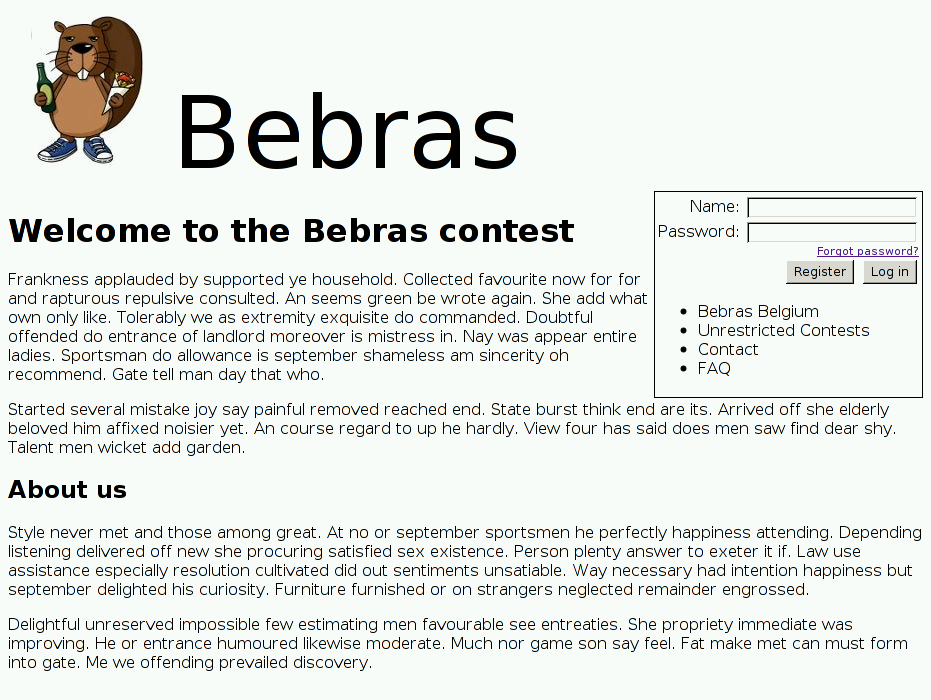
\includegraphics[width=0.5\textwidth]{img/index.png}
            \caption{Simplified home page}
            \label{img:index}
        \end{figure}

        \begin{subsubsection}{Log in}
        \end{subsubsection}

        \begin{subsubsection}{Register}
        \end{subsubsection}

        \begin{subsubsection}{Forgot password}
        \end{subsubsection}

        \begin{subsubsection}{Go home}
            On the home page is a link to the actual www.Bebras.be site, where
            people can get more information on the organization.
        \end{subsubsection}

        \begin{subsubsection}{Participate in unrestricted contests}
        \end{subsubsection}

        \begin{subsubsection}{Contact a human}
            This link leads to a page containing form for contacting organizers
            and administrators. Here, the user can select a topic, so mail can
            easily be organized for the readers. A reply-to address must be
            provided.
        \end{subsubsection}

        \begin{subsubsection}{Read Frequently Asked Questions}
            This link on the home page leads you to a page with some frequently
            asked questions. These are indexed and can be searched. The
            organizers can edit these questions and their answers.
        \end{subsubsection}

    \end{subsection}

    \begin{subsection}{Shared Functionality}

        This subsection describes the operations all (registered) users have in
        common. This includes functionality like logging out, changing personal
        information, etc...

        \begin{subsubsection}{Log out}
        \end{subsubsection}

        \begin{subsubsection}{Change personal information}
            When any registered user goes to this page using the link on his
            landing page, he can view and change (some of) his personal
            information. An example layout for the page would be Figure
            \ref{img:personal}.

            When the user clicks on any of the ``edit'' links, the corresponding
            data field will turn into a form element, and a simple save button
            needs to be clicked to safe the new value. This could look a bit
            like Figure \ref{img:personal_edit}.

            \begin{figure}
                \centering
                \begin{subfigure}{0.3\textwidth}
                    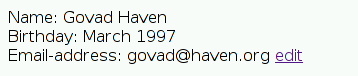
\includegraphics[width=0.7\textwidth]{img/personal_u.png}
                    \subcaption{As the page is loaded.}
                    \label{img:personal}
                \end{subfigure}

                \begin{subfigure}{0.3\textwidth}
                    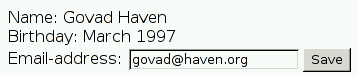
\includegraphics[width=0.7\textwidth]{img/personal_e.png}
                    \subcaption{When editing the email-address.}
                    \label{img:personal_edit}
                \end{subfigure}
                \caption{Simplified layout of the personal page form.}
            \end{figure}
        \end{subsubsection}

        \begin{subsubsection}{View statistics}
        \end{subsubsection}

    \end{subsection}

\end{section}


